\documentclass{article} 
\usepackage[left=0.75in,top=0.6in,right=0.75in,bottom=0.6in]{geometry} % Document margins
\usepackage{tabularx}
\usepackage{fancyvrb}
\usepackage{graphicx}
\usepackage{multicol,caption}
\usepackage{fancyhdr}
\usepackage{lipsum}
\usepackage{mathtools}
\usepackage{float}
\usepackage{textcomp}

%Header Stuff
\newenvironment{Figure}
  {\par\medskip\noindent\ignorespaces\minipage{\linewidth}}
  {\endminipage\par\medskip}

\usepackage{fancyhdr}
\pagestyle{fancy}
\fancyhf{}
\renewcommand{\headrulewidth}{0pt}
\fancyhead[R]{\thepage}


\begin{document}

%----------------------------------------------------------------------------------------
%		 TITLE 
%----------------------------------------------------------------------------------------
\begin{center}

\vspace* {15 pt}
\Huge{\bf Implementing AND gates, 8-bit binary counters and 2-Digit BCD counters using DE2-115 FPGA  }\\
\vspace {20 pt}
\large{Howard Edwards, Michael Micros, Jonathon  Rigney, Megan Rowland \\}

\end{center}

\vspace{20 pt}




\begin{multicols*}{2}

%----------------------------------------------------------------------------------------
%		ABSTRACT
%----------------------------------------------------------------------------------------
{\bf  \textit {Abstract(Jonathon Rigney)} ---
}\\
This report covers the development of three separate programs written for the Altera DE2-115 FPGA using the Cyclone 4 processor.These programs are written in VHDL then synthesised onto the board. The first of these programs creates an and gate using two of the onboard switches with an LED for output. The Second program is 8 bit binary up counter that is advanced by an onboard push button whose output is displayed on 8 LEDs. The final program is a two digit (0-99) Binary Coded Decimal counter. This program uses the previous push button to advance the counter and the output is displayed on two seven segments displays on the board.


{\bf  \textit {Index Terms} --- FPGA, 8-bit counter, Seven Segment Display
}



%----------------------------------------------------------------------------------------
%		INTRODUCTION
%----------------------------------------------------------------------------------------

\begin{center}
\large{I. Introduction(Howard Edwards)}
\end{center}
A vital aspect of a larger project is discussed in this paper. The project comprises of an integrated system that performs real-time video processing through an user-interface on a computer. This project is completed through the use of field-programmable gating arrays, FPGAs. As this is the case, FPGA familiarization is the main focus of this document. Three programs were created to facilitate the familiarization and operations of a FPGA and its subsequent design software, Quartus II.
The FPGA board used was Terasic Altera DE2-115. The board is comprised of the Altera Cyclone IV 4CE115 FPGA and other hardwares, like various memory types, LCD module, clocks, slide switches, pushbuttons and LEDs, to facilitate the implementation of a wide range of designed circuitries and projects. In order to use the DE2-115 board, the Quartus II software was used. Quartus II supports various design entry methods including Verilog, VHSIC Hardware Description Language (VHDL) and schematic entry. Specific features of the DE2-115 board and Quartus can be view in their respective user manuals.
All programs were written in VHDL to program the DE2-115 board. VHDL is a high-level programming language that the Quartus II software can automatically convert into a FPGA design. Each program was designed to utilize some basic function of the FPGA board. First program uses two slide switches as inputs for an AND gate then displays the output with one of the LEDs. Second program uses a push button as input for an 8-bit counter and display the counter value on 8 of the LEDs. The third uses a push button as input for a two-digit, binary-coded decimal counter (BCD) and display the value of the counter using two of the board's seven-segment displays. All programs were successfully written in VHDL, loaded onto the DE2-115 via the Quartus II software and functioned as intended.


%----------------------------------------------------------------------------------------
%		DESIGN
%----------------------------------------------------------------------------------------

\begin{center}
{\large II. Design (Michael Micros)}
\end{center}

{\bf A. Summary of Design--}  
The overall design consists of 3 Quartus projects that are loaded into the Altera DE2-115 FPGA and perform the following tasks:
Use two slide switches as inputs for an AND gate, display the output with one of the LEDs
Use a push button as input for a 8-bit counter and display the counter value on 8 of the LEDs.
Use a push button as input for a two-digit, binary-coded decimal counter (BCD) and display the value of the counter using two of the board's seven-segment displays.
All the projects contain VHDL files that are compiled and loaded to the FPGA in order to provide the desired functionality.


{\bf B. Detail Description}

{\bf AND gate using switches:} 
To create the functionality of an AND gate using the FPGA switches requires 2 simple tasks. Implementing the VHDL code for an AND gate using a concurrent statement --as seen in Fig1.-- and assigning 2 switches to the inputs x1, x2 and an LED to the output f.

\begin{Figure}
 \centering
 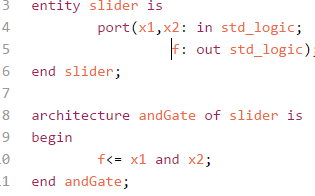
\includegraphics[height = 4 cm]{slider.png}
  \captionof{figure}{VHDL code that implements an AND gate}
\end{Figure}
  

{\bf 8-bit counter using pushbutton and LEDs:} \\
In order to implement the 8-bit counter in VHDL, the VHDL entity consists of 1 std\_logic input "x1" corresponding to the pushbutton, and an unsigned(0 to 7) vector “f” that corresponds to the 8 LEDs that will display the result.


\begin{Figure}
 \centering
 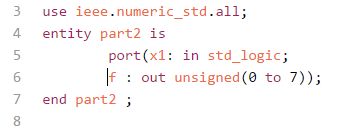
\includegraphics[width=\linewidth]{p2entity.png}
  \captionof{figure}{VHDL code for the 8-bit counter entity}
\end{Figure}

The VHDL program displayed below makes use of an integer named “cnt” which is initialized to zero and incremented every time the pushbutton is pressed. The pushbutton signal is active low, therefore a value of 0 indicates that the pushbutton is being pressed. When the counter is incremented modulo 264 (in order for the counter to wrap around), the integer value of “cnt” is converted to an 8 bit unsigned vector and stored into the output vector ”f”. The final step that must be taken is to assign pins to the input and output variables, by going to "Assignments" \textrightarrow "Pin Planner". Key 1 was selected as the pushbutton, since key 0 was defective on the board being used, and LEDG[10]-LEDG[17] were used to display the state of the counter.

\begin{Figure}
 \centering
 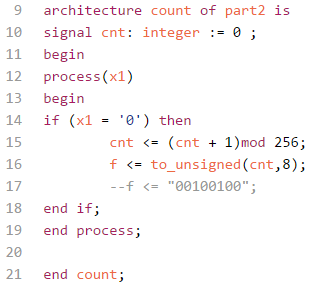
\includegraphics[width=\linewidth]{p2code.png}
  \captionof{figure}{VHDL code for the 8-bit counter entity}
\end{Figure}



{\bf Two-digit, binary-coded decimal counter using seven segment displays:}\\
The VHDL entity for the BCD counter consists of  1 std\_logic input “x1” corresponding to the pushbutton, and 2 unsigned(0 to 6) output vectors “f0” and f1 corresponding to the 2 seven segment displays. Similarly, to the 8-bit counter a counter “cnt is used and is made to wrap around at 100. “Cnt” is initialized at 0 and incremented by the the pushbutton, which operates in the same exact fashion as in the 8-bit counter. Two variables (msd and lsd) are used to store the most significant digits and least significant digits of “cnt” by isolating the quotient and the remainder.\\

\begin{Figure}
 \centering
 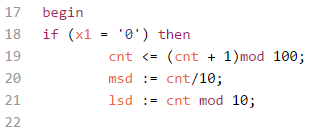
\includegraphics[width=\linewidth]{p3c1.png}
  \captionof{figure}{VHDL code showing how to obtain the most significant and least significant digits}
\end{Figure}

The results will always be in the range 0 to 9, and based on that value, the appropriate 7-bit vector is stored into the output vectors “f0 and “f1”.\\
Similarly to the 8-bit counter, the pushbutton was assigned to Key 1 and the seven segments displays that were used were HEX6[] and HEX7.


\begin{Figure}
 \centering
 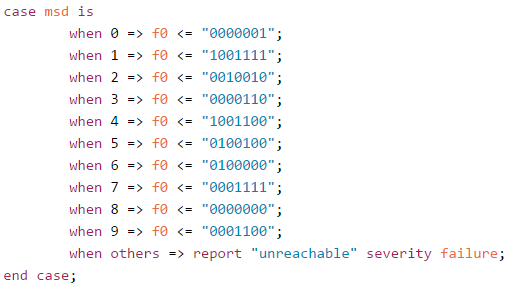
\includegraphics[width=\linewidth]{msd.png}
  \captionof{figure}{VHDL code showing how the output vector is set based on the decimal value of "msd"}
\end{Figure}

\begin{Figure}
 \centering
 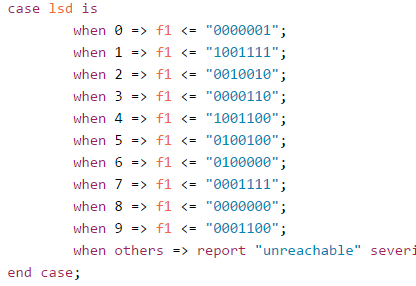
\includegraphics[width=\linewidth]{lsd.png}
  \captionof{figure}{VHDL code showing how the output vector is set based on the decimal value of "lsd"}
\end{Figure}



%----------------------------------------------------------------------------------------
%		EVALUATION
%----------------------------------------------------------------------------------------

\begin{center}
{\large III. Evaluation (Megan Rowland)}\\
\end{center}

The AND gate is the combination of two switches and one LED. When both switches are switched to the on position, the LED lights up. Otherwise, the LED does not light up.

The 8-bit counter is a combination of a push button and eight LEDs. When the push button is pressed, the eight LEDs begin to light up as the 8-bit binary representation of the count. When the 8-bit counter reaches 255, the next press of the button starts the count back at zero. The following pictures show the binary representation of the 8-bit counter at 93, 255 and 1 respectively:

\begin{Figure}
 \centering
 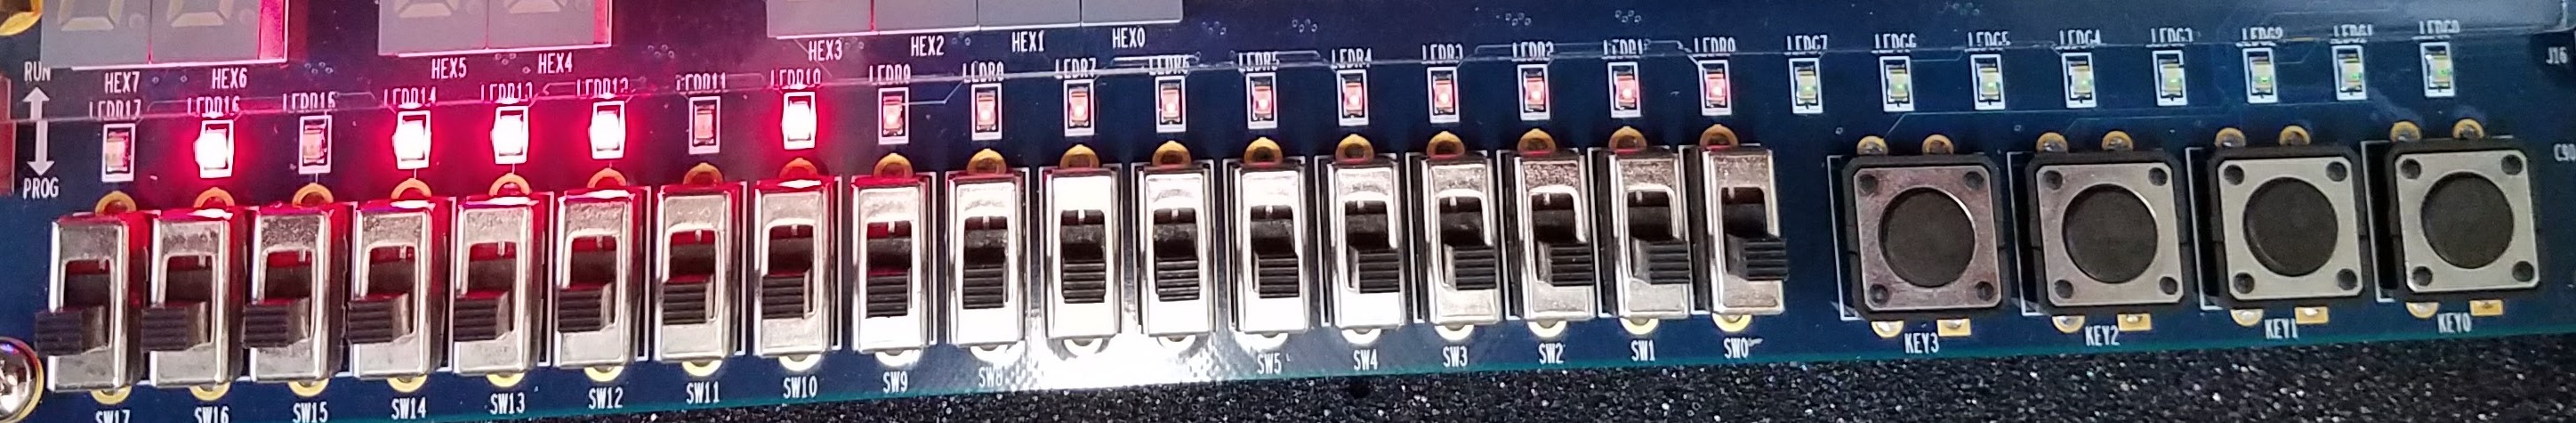
\includegraphics[width=\linewidth]{Binary93.jpg}
  \captionof{figure}{Counter = 93}
\end{Figure}

\begin{Figure}
 \centering
 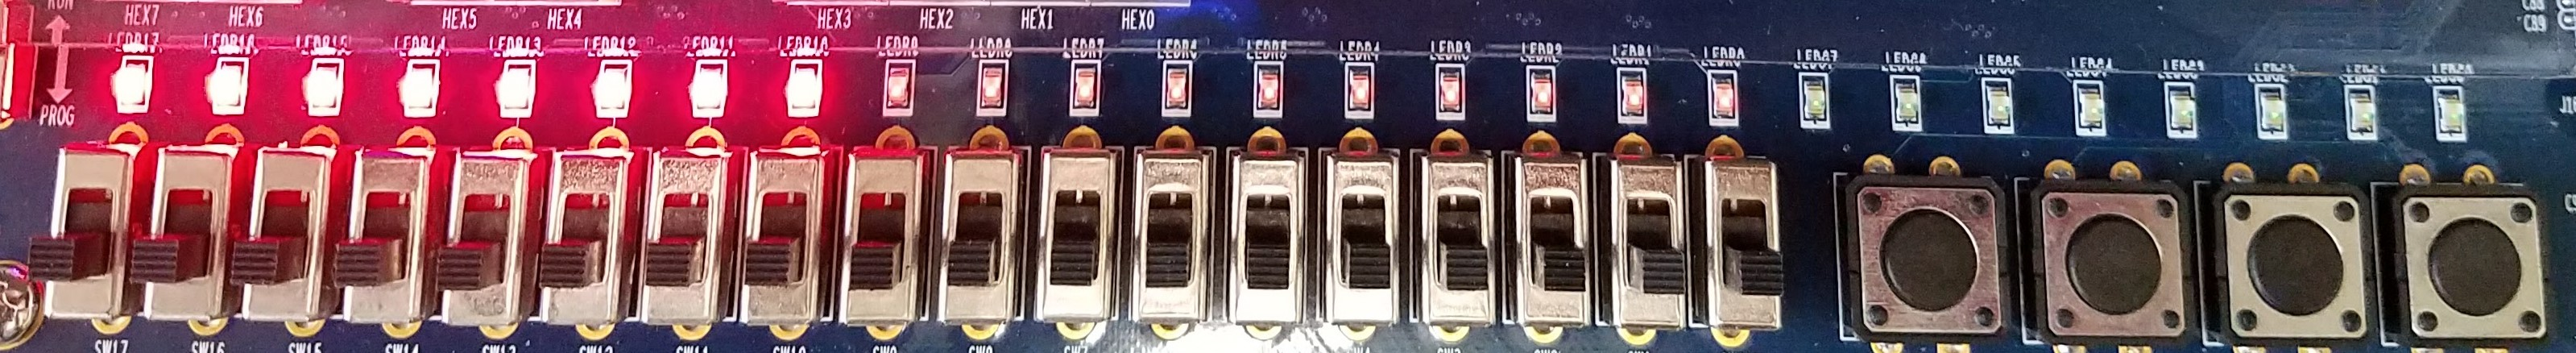
\includegraphics[width=\linewidth]{Binary255.jpg}
  \captionof{figure}{Counter = 255}
\end{Figure}

\begin{Figure}
 \centering
 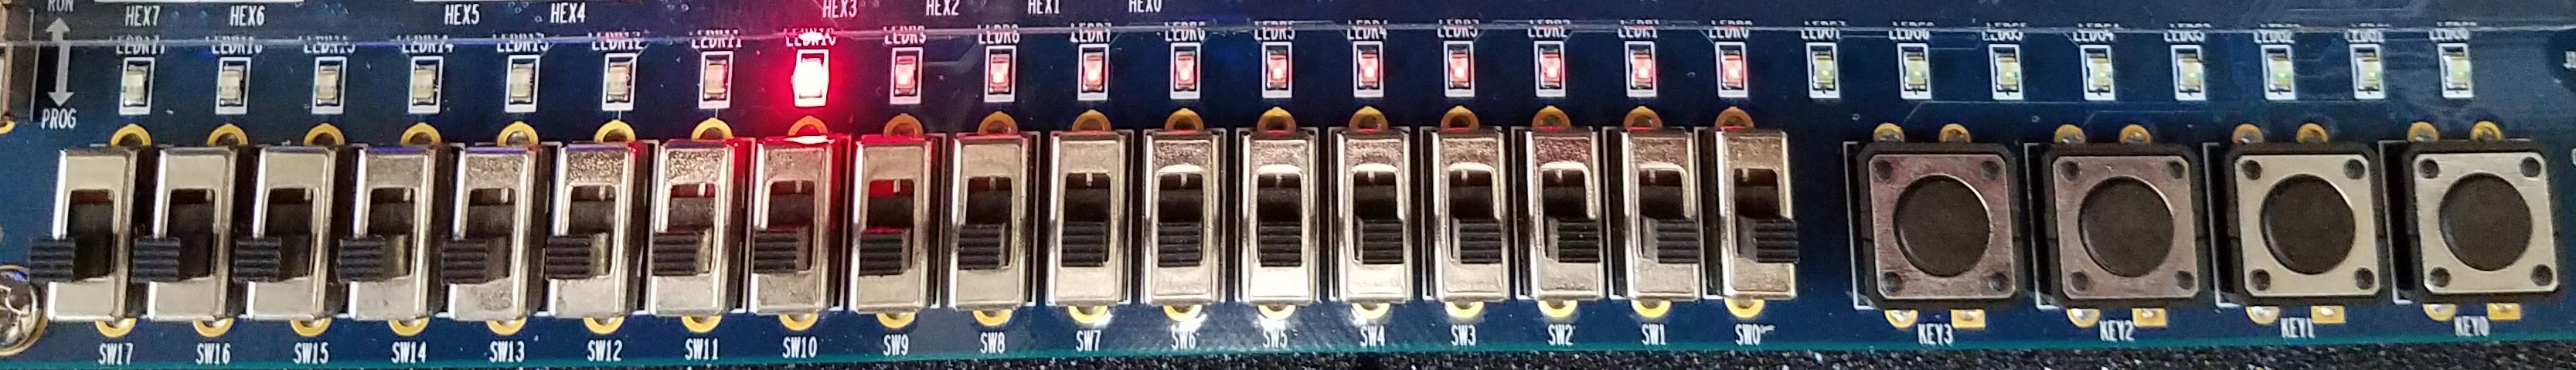
\includegraphics[width=\linewidth]{Binary1.jpg}
  \captionof{figure}{Counter = 1 after wrap around }
\end{Figure}


The two-digit counter is a combination of a push button and two of the seven-segment displays. When the push button is pressed, the two-digit display presents the decimal representation of the count. When the two-digit display reaches 99, the next press of the button starts the count back at zero. The following pictures show the decimal representation of the two-digit counter at 63, 99 and 0 respectively:

\begin{Figure}
 \centering
 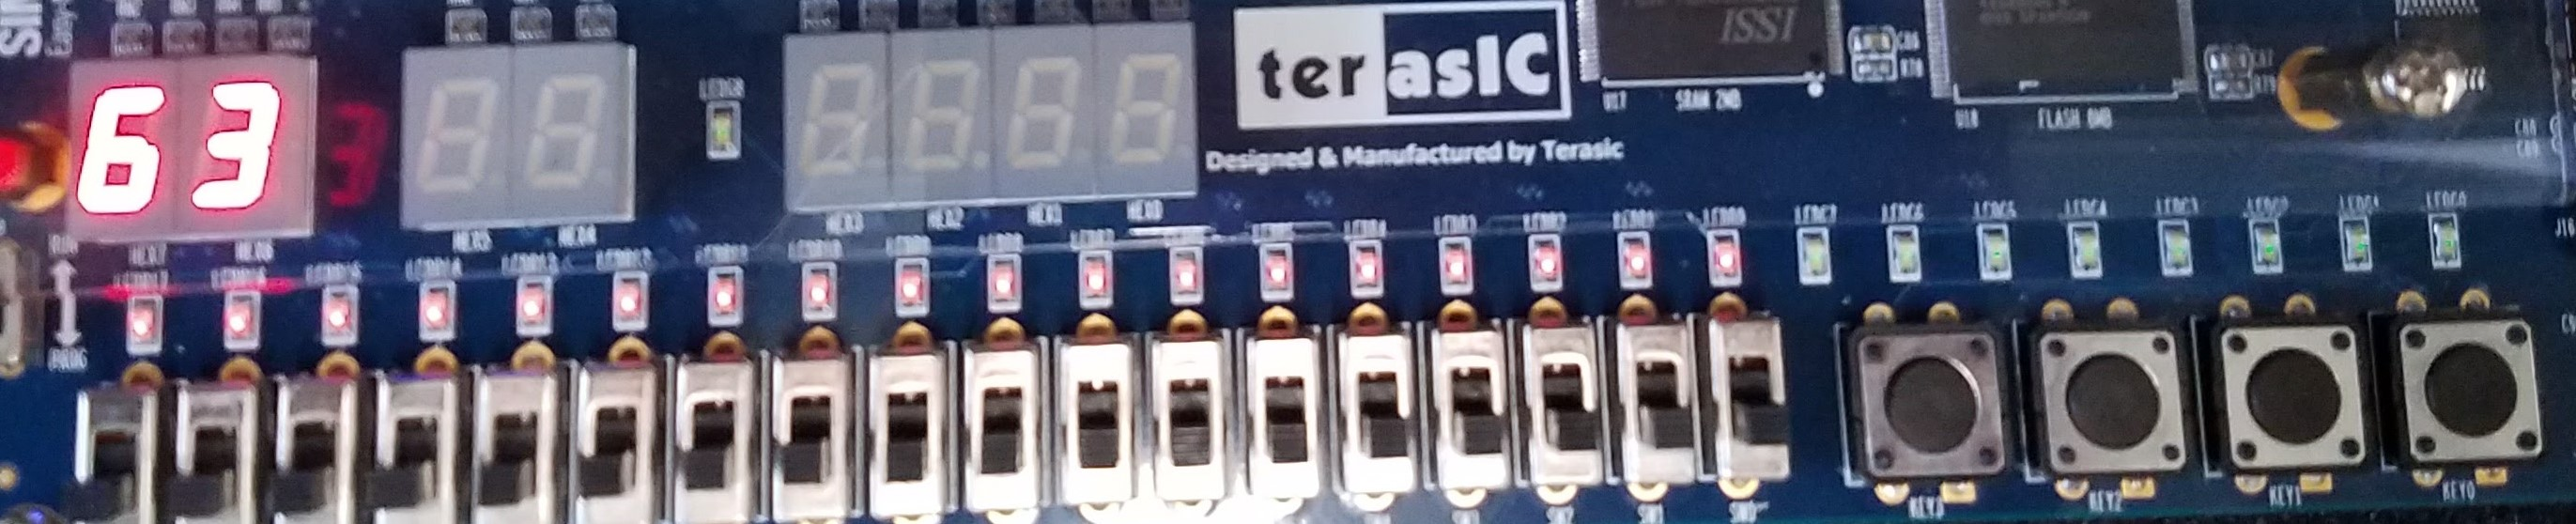
\includegraphics[width=\linewidth]{Digital63.jpg}
  \captionof{figure}{Counter = 63}
\end{Figure}

\begin{Figure}
 \centering
 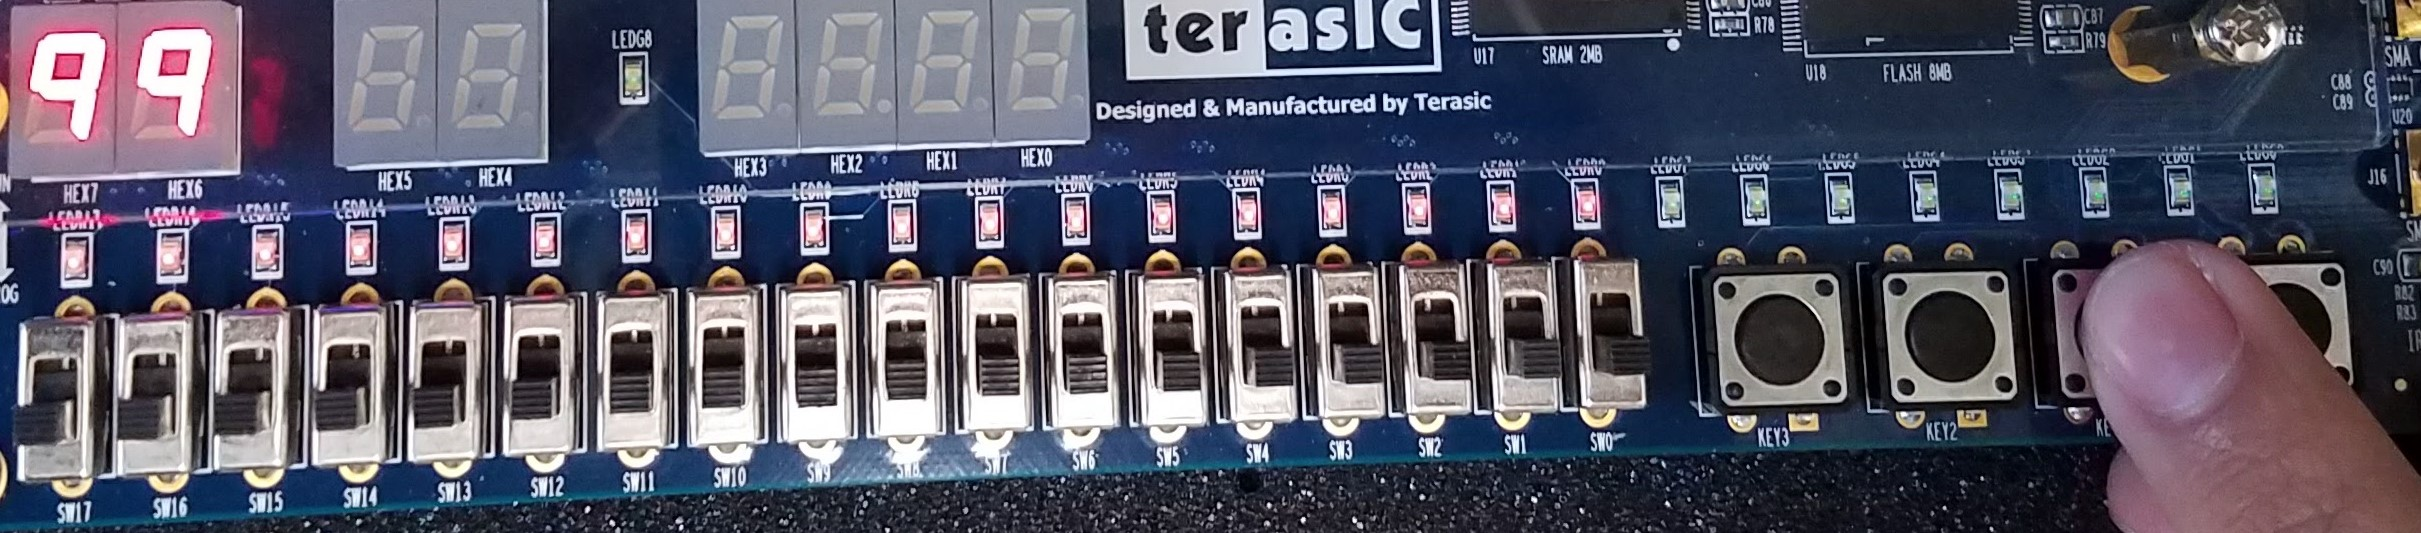
\includegraphics[width=\linewidth]{Digital99.jpg}
  \captionof{figure}{Counter = 99}
\end{Figure}

\begin{Figure}
 \centering
 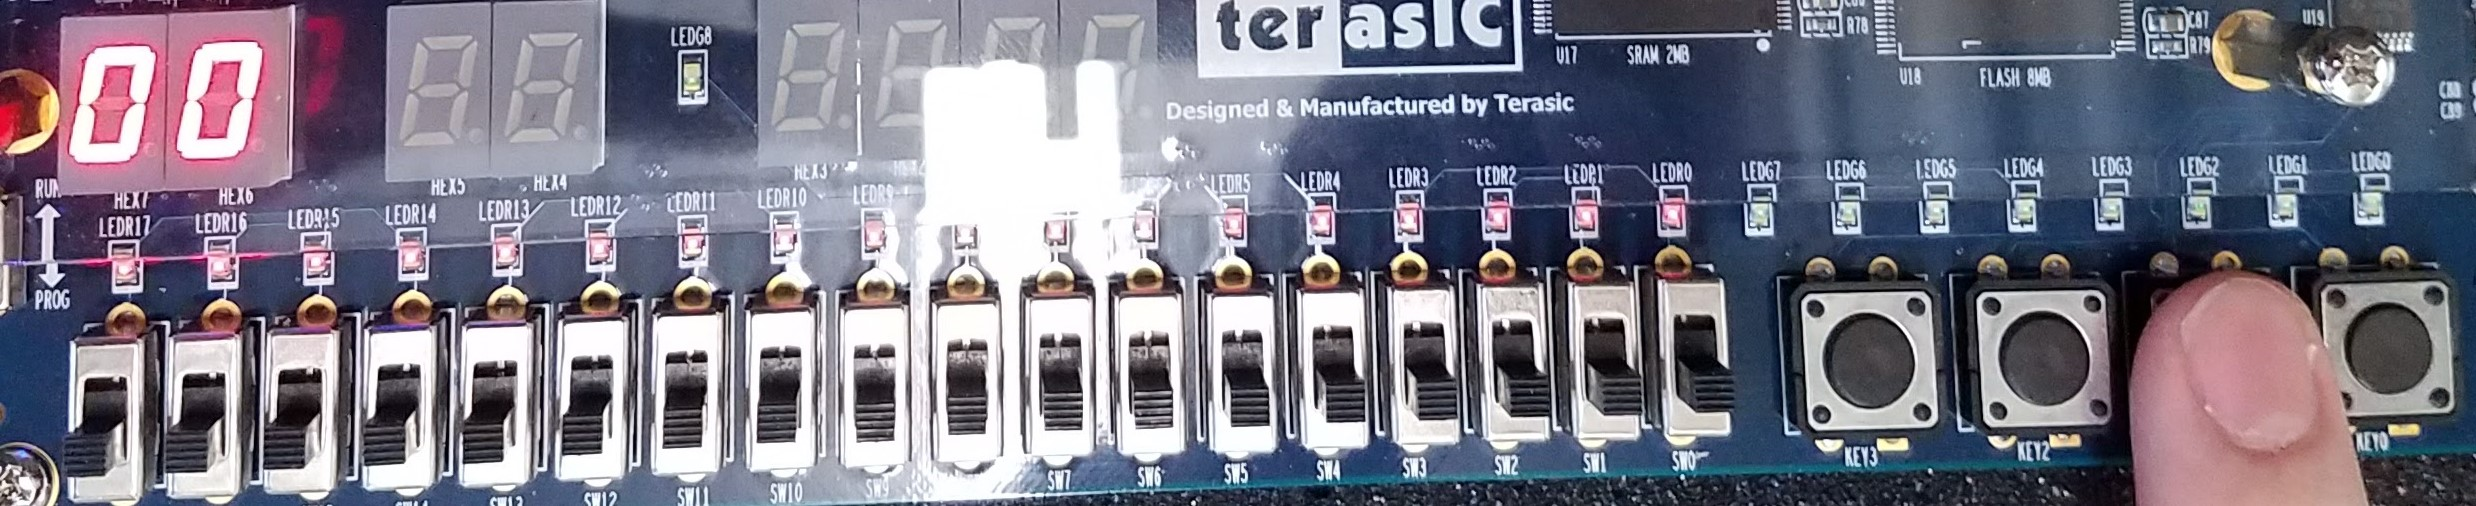
\includegraphics[width=\linewidth]{Digital00.jpg}
  \captionof{figure}{Counter = 00 after wrap around}
\end{Figure}


\vspace{15 pt}

%----------------------------------------------------------------------------------------
%		DISCUSSION
%----------------------------------------------------------------------------------------


\begin{center}
{\large IV. Discussion (Megan Rowland)}
\end{center}
Based on the Evaluation section, the three vhdl programs (AND gate, 8-bit counter, and two-digit counter) function as discussed. There is not much room for improvement. There was no sign of issues with the push button bouncing, so there was no need to implement debouncing code for the push button.
For the AND gate, when the switches are put in the on position, the LED immediately lights. For the 8-bit counter, as soon as the push button is pressed the binary counter increases by one and displays on the LEDs. When the count is at the maximum number, 255, the next press of the button starts the counter back at 0 and displays the binary value on the LEDs. For the two-digit counter, as soon as the push button is pressed the counter increases by one and displays on two of the seven-segment displays. When the count is at the maximum number, 99, the next press of the button starts the counter back at 0 and displays the decimal value on two of the seven-segment displays.


%----------------------------------------------------------------------------------------
%		APPENDIX
%----------------------------------------------------------------------------------------


\begin{center}
{\large V. Appendix}
\end{center}

\end{multicols*}













%----------------------------------------------------------------------------------------
\end{document}
